\documentclass{standalone}
\usepackage{tikz}
\usetikzlibrary{patterns, positioning}
\usepackage[sfdefault]{ClearSans} %% option 'sfdefault' activates Clear Sans as the default text font
\usepackage[T1]{fontenc}

\begin{document}
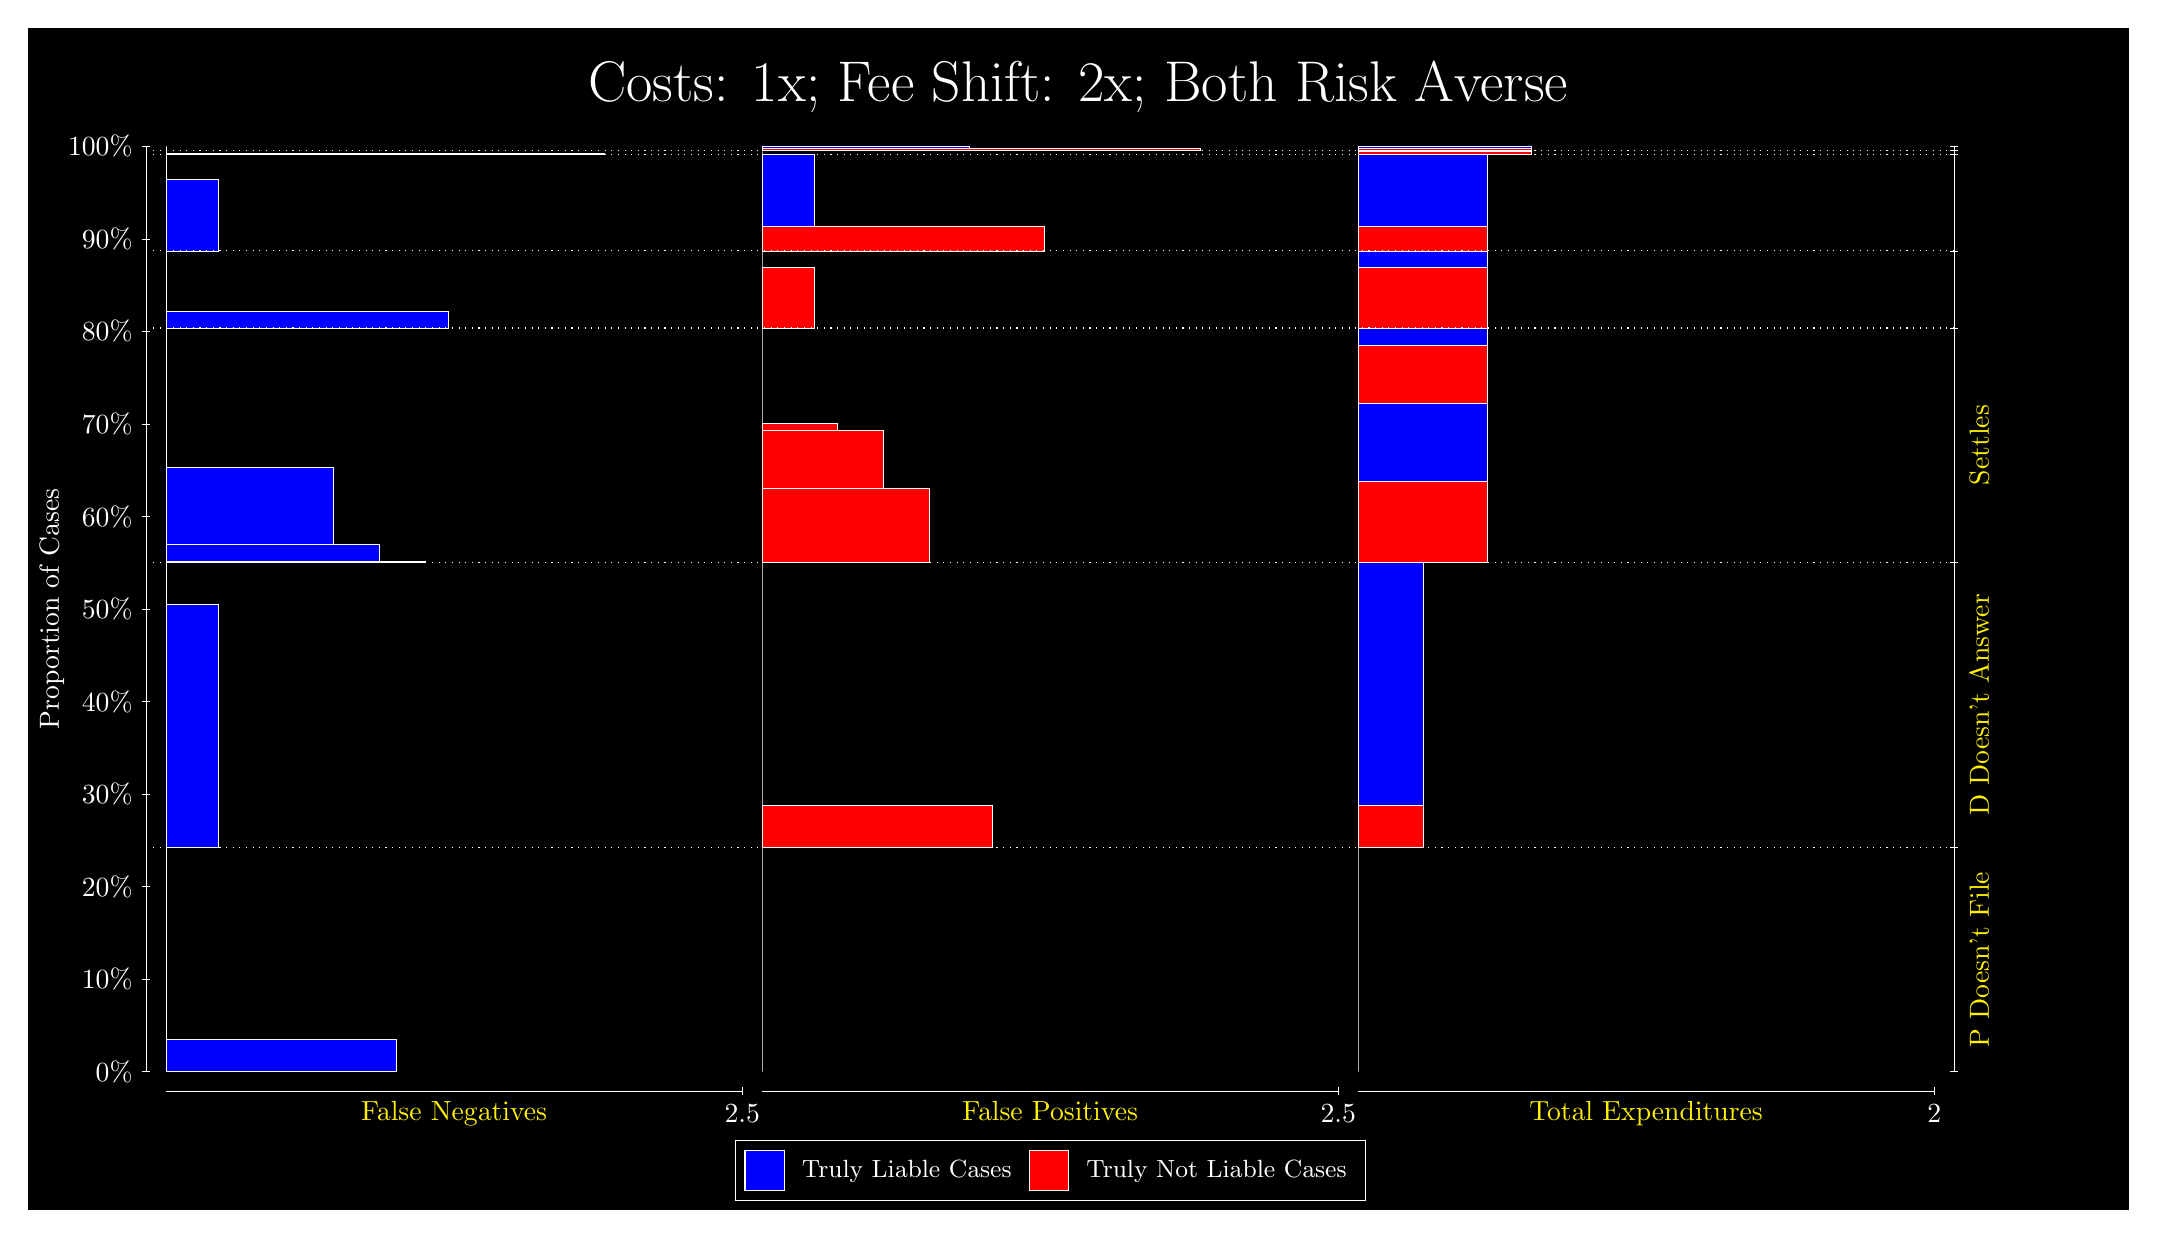
\begin{tikzpicture}
\draw[fill=black] (0,0) rectangle (26.667,15);
\draw[text=white] (0,13.5) rectangle (26.667,15) node[midway] {\huge Costs: 1x; Fee Shift: 2x; Both Risk Averse};
\draw[white, very thin] (1.5,1.75) -- (1.5,13.5);
\node[rotate=90, text=white, anchor=center] at (0.3, 7.625) {Proportion of Cases};
\draw[white, very thin] (1.45,1.75) -- (1.55,1.75);
\node[text=white, anchor=east] at (1.45, 1.75) {0\%};
\draw[white, very thin] (1.45,2.925) -- (1.55,2.925);
\node[text=white, anchor=east] at (1.45, 2.925) {10\%};
\draw[white, very thin] (1.45,4.1) -- (1.55,4.1);
\node[text=white, anchor=east] at (1.45, 4.1) {20\%};
\draw[white, very thin] (1.45,5.275) -- (1.55,5.275);
\node[text=white, anchor=east] at (1.45, 5.275) {30\%};
\draw[white, very thin] (1.45,6.45) -- (1.55,6.45);
\node[text=white, anchor=east] at (1.45, 6.45) {40\%};
\draw[white, very thin] (1.45,7.625) -- (1.55,7.625);
\node[text=white, anchor=east] at (1.45, 7.625) {50\%};
\draw[white, very thin] (1.45,8.8) -- (1.55,8.8);
\node[text=white, anchor=east] at (1.45, 8.8) {60\%};
\draw[white, very thin] (1.45,9.975) -- (1.55,9.975);
\node[text=white, anchor=east] at (1.45, 9.975) {70\%};
\draw[white, very thin] (1.45,11.15) -- (1.55,11.15);
\node[text=white, anchor=east] at (1.45, 11.15) {80\%};
\draw[white, very thin] (1.45,12.325) -- (1.55,12.325);
\node[text=white, anchor=east] at (1.45, 12.325) {90\%};
\draw[white, very thin] (1.45,13.5) -- (1.55,13.5);
\node[text=white, anchor=east] at (1.45, 13.5) {100\%};

\draw[white, very thin] (24.457,1.75) -- (24.457,13.5);
\draw[white, very thin] (24.407,1.75) -- (24.507,1.75);
\node[anchor=west] at (24.407, 1.75) {};
\draw[white, very thin] (24.407,4.5927) -- (24.507,4.5927);
\node[anchor=west] at (24.407, 4.5927) {};
\draw[white, very thin] (24.407,8.2173) -- (24.507,8.2173);
\node[anchor=west] at (24.407, 8.2173) {};
\draw[white, very thin] (24.407,11.193) -- (24.507,11.193);
\node[anchor=west] at (24.407, 11.193) {};
\draw[white, very thin] (24.407,12.172) -- (24.507,12.172);
\node[anchor=west] at (24.407, 12.172) {};
\draw[white, very thin] (24.407,13.393) -- (24.507,13.393);
\node[anchor=west] at (24.407, 13.393) {};
\draw[white, very thin] (24.407,13.452) -- (24.507,13.452);
\node[anchor=west] at (24.407, 13.452) {};
\draw[white, very thin] (24.407,13.5) -- (24.507,13.5);
\node[anchor=west] at (24.407, 13.5) {};

\draw[white, very thin, fill=blue] (1.75,1.75) rectangle (4.6775,2.162);
\draw[white, very thin, fill=red] (1.75,2.162) rectangle (1.75,4.5927);
\draw[white, very thin, fill=blue] (1.75,4.5927) rectangle (2.4087,7.6824);
\draw[white, very thin, fill=red] (1.75,7.6824) rectangle (1.75,8.2173);
\draw[white, very thin, fill=blue] (1.75,8.2173) rectangle (5.0435,8.2292);
\draw[white, very thin, fill=blue] (1.75,8.2292) rectangle (4.458,8.4487);
\draw[white, very thin, fill=blue] (1.75,8.4487) rectangle (3.8725,9.426);
\draw[white, very thin, fill=red] (1.75,9.426) rectangle (1.75,11.193);
\draw[white, very thin, fill=blue] (1.75,11.193) rectangle (5.3362,11.401);
\draw[white, very thin, fill=red] (1.75,11.401) rectangle (1.75,12.172);
\draw[white, very thin, fill=blue] (1.75,12.172) rectangle (2.4087,13.08);
\draw[white, very thin, fill=red] (1.75,13.08) rectangle (1.75,13.393);
\draw[white, very thin, fill=blue] (1.75,13.393) rectangle (7.3123,13.41);
\draw[white, very thin, fill=red] (1.75,13.41) rectangle (1.75,13.452);
\draw[white, very thin, fill=red] (1.75,13.452) rectangle (1.75,13.469);
\draw[white, very thin, fill=blue] (1.75,13.469) rectangle (1.75,13.5);
\draw[white, very thin, fill=red] (9.3189,1.75) rectangle (9.3189,4.1807);
\draw[white, very thin, fill=blue] (9.3189,4.1807) rectangle (9.3189,4.5927);
\draw[white, very thin, fill=red] (9.3189,4.5927) rectangle (12.246,5.1276);
\draw[white, very thin, fill=blue] (9.3189,5.1276) rectangle (9.3189,8.2173);
\draw[white, very thin, fill=red] (9.3189,8.2173) rectangle (11.441,9.1605);
\draw[white, very thin, fill=red] (9.3189,9.1605) rectangle (10.856,9.8996);
\draw[white, very thin, fill=red] (9.3189,9.8996) rectangle (10.27,9.9848);
\draw[white, very thin, fill=blue] (9.3189,9.9848) rectangle (9.3189,11.193);
\draw[white, very thin, fill=red] (9.3189,11.193) rectangle (9.9776,11.964);
\draw[white, very thin, fill=blue] (9.3189,11.964) rectangle (9.3189,12.172);
\draw[white, very thin, fill=red] (9.3189,12.172) rectangle (12.905,12.484);
\draw[white, very thin, fill=blue] (9.3189,12.484) rectangle (9.9776,13.393);
\draw[white, very thin, fill=red] (9.3189,13.393) rectangle (9.3189,13.434);
\draw[white, very thin, fill=blue] (9.3189,13.434) rectangle (9.3189,13.452);
\draw[white, very thin, fill=red] (9.3189,13.452) rectangle (14.881,13.469);
\draw[white, very thin, fill=blue] (9.3189,13.469) rectangle (11.954,13.5);
\draw[white, very thin, fill=red] (16.888,1.75) rectangle (16.888,4.1807);
\draw[white, very thin, fill=blue] (16.888,4.1807) rectangle (16.888,4.5927);
\draw[white, very thin, fill=red] (16.888,4.5927) rectangle (17.711,5.1276);
\draw[white, very thin, fill=blue] (16.888,5.1276) rectangle (17.711,8.2173);
\draw[white, very thin, fill=red] (16.888,8.2173) rectangle (18.534,9.2457);
\draw[white, very thin, fill=blue] (16.888,9.2457) rectangle (18.534,10.235);
\draw[white, very thin, fill=red] (16.888,10.235) rectangle (18.534,10.974);
\draw[white, very thin, fill=blue] (16.888,10.974) rectangle (18.534,11.193);
\draw[white, very thin, fill=red] (16.888,11.193) rectangle (18.534,11.964);
\draw[white, very thin, fill=blue] (16.888,11.964) rectangle (18.534,12.172);
\draw[white, very thin, fill=red] (16.888,12.172) rectangle (18.534,12.484);
\draw[white, very thin, fill=blue] (16.888,12.484) rectangle (18.534,13.393);
\draw[white, very thin, fill=red] (16.888,13.393) rectangle (19.083,13.434);
\draw[white, very thin, fill=blue] (16.888,13.434) rectangle (19.083,13.452);
\draw[white, very thin, fill=red] (16.888,13.452) rectangle (19.083,13.469);
\draw[white, very thin, fill=blue] (16.888,13.469) rectangle (19.083,13.5);
\draw[white, dotted] (1.5,4.5927) -- (24.457,4.5927);
\draw[white, dotted] (1.5,8.2173) -- (24.457,8.2173);
\draw[white, dotted] (1.5,11.193) -- (24.457,11.193);
\draw[white, dotted] (1.5,12.172) -- (24.457,12.172);
\draw[white, dotted] (1.5,13.393) -- (24.457,13.393);
\draw[white, dotted] (1.5,13.452) -- (24.457,13.452);
\draw[white, very thin] (1.75,1.5) -- (9.0689,1.5);
\node[text=yellow, anchor=north] at (5.4094, 1.5) {False Negatives};
\draw[white, very thin] (9.0689,1.45) -- (9.0689,1.55);
\node[text=white, anchor=north] at (9.0689, 1.45) {2.5};

\draw[white, very thin] (9.3189,1.5) -- (16.638,1.5);
\node[text=yellow, anchor=north] at (12.978, 1.5) {False Positives};
\draw[white, very thin] (16.638,1.45) -- (16.638,1.55);
\node[text=white, anchor=north] at (16.638, 1.45) {2.5};

\draw[white, very thin] (16.888,1.5) -- (24.207,1.5);
\node[text=yellow, anchor=north] at (20.547, 1.5) {Total Expenditures};
\draw[white, very thin] (24.207,1.45) -- (24.207,1.55);
\node[text=white, anchor=north] at (24.207, 1.45) {2};

\node[text=yellow, centered, rotate=90] at (24.777, 3.1713) {P Doesn't File};
\node[text=yellow, centered, rotate=90] at (24.777, 6.405) {D Doesn't Answer};
\node[text=yellow, centered, rotate=90] at (24.777, 9.7054) {Settles};





\draw (12.978300999999998,1.5) node[draw=none] (baseCoordinate) {};
\begin{scope}[align=center]
        \matrix[scale=0.5, draw=white, below=0.5cm of baseCoordinate, nodes={draw}, column sep=0.1cm]{
            \node[rectangle, draw, minimum width=0.5cm, minimum height=0.5cm, fill=blue] {}; &
            \node[draw=none, font=\small, text=white] (B) {Truly Liable Cases}; &
            \node[rectangle, draw, minimum width=0.5cm, minimum height=0.5cm, fill=red] {}; &
            \node[draw=none, font=\small, text=white] (B) {Truly Not Liable Cases}; \\
            };
\end{scope}

\end{tikzpicture}
\end{document}